\documentclass[maincolor=black]{exercise}
\settitle[Projektteil 3]{Algorithmik}
\addstudent[625391]{Kaspar-David Buss}
\addstudent[573537]{Julian Hoffmann}
\setgroup{Gruppe 2 (Mittwochsgruppe)}
\setlength{\parskip}{0em}
\setlength{\parindent}{3ex}
\usepackage[utf8]{inputenc}
\usepackage[]{listings}
\usepackage{algorithm}
\usepackage{algorithmic}
\usepackage{enumitem}
\usepackage{booktabs}
\usepackage{changepage}

\lstset{literate=%
	{Ö}{{\"O}}1
	{Ä}{{\"A}}1
	{Ü}{{\"U}}1
	{ß}{{\ss}}1
	{ü}{{\"u}}1
	{ä}{{\"a}}1
	{ö}{{\"o}}1
	{~}{{\textasciitilde}}1
}

\newcommand{\anf}[1]{„#1“}
\newcommand{\non}[1]{\overline{#1}}

\begin{document}
\section*{Vorgehensweise}
Wir haben eine Lösung dieser Aufgabe in Java implementiert. Unsere Implementation besteht aus verschiedenen Teilen, welche die einzelnen Aufgaben erfüllen.\par
Das erste Modul führt den Modified-3-SAT-Algorithmus für eine bestimmte Formel aus. Das zweite Modul führt, beginnend bei einer bestimmten Anzahl von Variablen und einer Verteilung $[i]$, die Suche nach $n_{max}$ und $m_3^{[i]}(n)$ aus. Das dritte Modul berechnet die Werte von $\sigma_3^{[i]}(n_{max},m)$, wenn $m$ um höchstens 10\% von $m_3^{[i]}(n_{max})$ abweicht. Diese werden wir in diesem Abschnitt etwas genauer behandeln.

\subsection{Solver}
Die Klasse \anf{\texttt{Solver}} in unserer Implementierung erhält als Eingabe eine bestimmte 3-KNF-Formel $\varphi$ mit $m$ Klauseln sowie die Anzahl der Variablen $\{x_1,x_2,...,x_n\}$. Intern ist eine solche Formel $\varphi$ bei uns ein Array von \texttt{int}-Werten der Größe $m \times 3$. Jedes Unterarray ist eine Klausel und die einzelnen Werte stehen für Literale. Ein positiver Wert $v$ steht hierbei für das Literal $x_v$, wohingegen ein negativer Wert $-v$ für das Literal $\non{x_v}$ steht.\par
Der Aufbau dieser Klasse besteht aus drei Ebenen. Die unterste Ebene ist eine Methode, die Random-3-SAT ausführt und als zusätzliche Eingabe $l$, die Anzahl an Iterationen erhält. Diese startet, wie angegeben, mit einer zufälligen Belegung von Variablen, die hierbei einfach ein \texttt{boolean}-Array der Länge $n$ ist. Der \texttt{return}-Wert dieser Methode ist eine erfüllende Belegung, falls eine solche gefunden wurde.\par
Die nächste Ebene ist eine Methode, welche Modifified-3-SAT ausführt und als zusätzliche Eingabe $r$, die Anzahl an Restarts erhält Wie angegeben, startet diese $r$-mal die Random-3-SAT-Methode mit $l = 3\cdot n$. Der \texttt{return}-Wert ist abermals eine erfüllende Belegung, falls eine solche gefunden wurde.\par
Schließlich gibt es noch eine \anf{\texttt{solve}}-Methode, die keine weiteren Eingaben erhält. Diese berechnet zuerst die benötigte Anzahl an Restarts, um eine Fehlerwahrscheinlichkeit von höchstens $10^{-13}$ zu erreichen, in unserem Fall $r = 60 \cdot \left(\frac{4}{3}\right)^n$, und führt Modified-3-SAT mit dieser Anzahl an Restarts aus. Falls eine erfüllende Belegung gefunden wurde, gibt diese \texttt{true} aus, sonst \texttt{false}.\par
Als Hilfsmethode ist noch eine Methode vorhanden, die überprüft, ob eine bestimmte Belegung die Formel erfüllt sowie eine Methode, die ein zufälliges Literal in einer der nicht erfüllten Klauseln auswählt und dessen Wert in der Belegung ändert.

\subsection{MassSolver}
Die Klasse \anf{\texttt{MassSolver}} in unserer Implementierung besteht wiederum aus drei Teilen. Jede dieser erhält als Eingabe immer die Zahl $i$ der Verteilung $[i]$, die angibt, wie die Klauseln generiert werden.\par
Die erste Ebene ist eine Methode, die als Eingabe ein bestimmtes Paar $(n,m)$ erhält. Es wird 100-mal eine zufällige Formel $\varphi$ mit $n$ Variablen und $m$ Klauseln generiert. Anschließend wird versucht, mittels \texttt{Solver} eine erfüllende Belegung von $\varphi$ zu finden. Nach diesen 100 Versuchen wird die durchschnittliche Zeit $t$ pro Erfüllbarkeitssuche sowie der Anteil $a$ an erfüllten Formeln zu 100 ermittelt und ausgegeben.\par
Die zweite Ebene ist eine Methode, die wiederum ein Paar $(n,m)$ erhält und an die erste Ebene weitergibt. Solange der oben genannte Anteil größer als $0.5$ ist, wird $m$ um 1 erhöht und $(n,m)$ abermals an die erste Ebene weitergegeben. Sobald der Anteil für ein $(n,m_s)$ aber kleiner als $0.5$ ist, werden dieser Anteil $a_s$ sowie der vorige $a_{s-1}$ ausgewählt und deren Abstand zu $0.5$ verglichen. Abhängig davon, welcher Abstand kleiner ist, wird entweder $m_s$ oder $m_{s-1}$ ausgegeben. Dies ist $m_3^{[i]}(n)$. Zusätzlich wird die letzte Ausgabe von Ebene 1 ausgegeben. Dies basiert auf der Annahme, dass $\sigma_3^{[i]}(n,m)$ monoton fallend in $m$ ist, was Sinn macht, da mehr Anforderungen an die Belegung gegeben sind und daher ein Erfolg unwahrscheinlicher ist. Ferner konnten wir dies durch unsere Experimente bestätigen.\par
Die dritte Ebene erhält lediglich einen Startwert $n := n_{start}$ als Eingabe und baut ein Mapping $M: n \mapsto m_3^{[i]}(n)$ auf. $m$ startet hierbei bei 1. Das Tupel $(n,m)$ wird an Ebene 2 weitergegeben und die Ausgabe wird betrachtet, womit $m_3^{[i]}(n)$ bestimmt ist und in $M$ eingetragen wird. Solange die in Ebene 1 ermittelte durchschnittliche Zeit $t$ kleiner als 3 Sekunden ist, wird $m := m_3^{[i]}(n)$ gesetzt, $n$ um 1 inkrementiert und $(n,m)$ abermals an Ebene 2 weitergegeben. Sobald aber $t$ größer als 3 Sekunden ist, bricht die Schleife ab und es wird $M$ ausgegeben. Dies basiert auf der Annahme, dass $m_3^{[i]}(n)$ monoton steigend ist, was Sinn macht, da für gleich bleibendes $m$ ein größeres $n$ mehr Freiheiten bietet, um Belegungen zu erstellen. Ferner konnten wir dies durch unsere Experimente bestätigen.\\
Diese Klasse enthält weiterhin Hilfsmethoden zur Generierung von zufälligen Formeln nach Verteilung $[1]$ oder $[2]$ sowie eine Methode, um aus einer Formel $\varphi$ triviale Klauseln, in denen $x \vee \non{x}$ für eine Variable $x$ vorkommt, sowie Duplikate von Klauseln zu entfernen. Letzteres verändert die Erfüllbarkeit der Formel nicht, macht aber die Erfüllbarkeitssuche deutlich schneller. Da die Klauseln \emph{unabhängig} aus der Verteilung $[i]$ gewählt werden, sind Duplikate nämlich noch nicht von vornherein ausgeschlossen.

Für Aufgabenteil b werden die Werte $n_{max}$, sowie die Anzahl der Klauseln $m_3^{[i]}(n_{max})$ aus Aufgabenteil a benutzt. Bei Variante 1 werden also die Wahrscheinlichkeiten für $n_{max} = 29$ und $m$ im Intervall [122,148] berechnet. Für die zweite Variante werden die Wahrscheinlichkeiten von $n_{max} = 27$ und $m$ im Intervall [111, 135] berechnet.

\section*{Ergebnisse}
\subsection{Aufgabe 3.3a)}
\begin{figure}[t]
	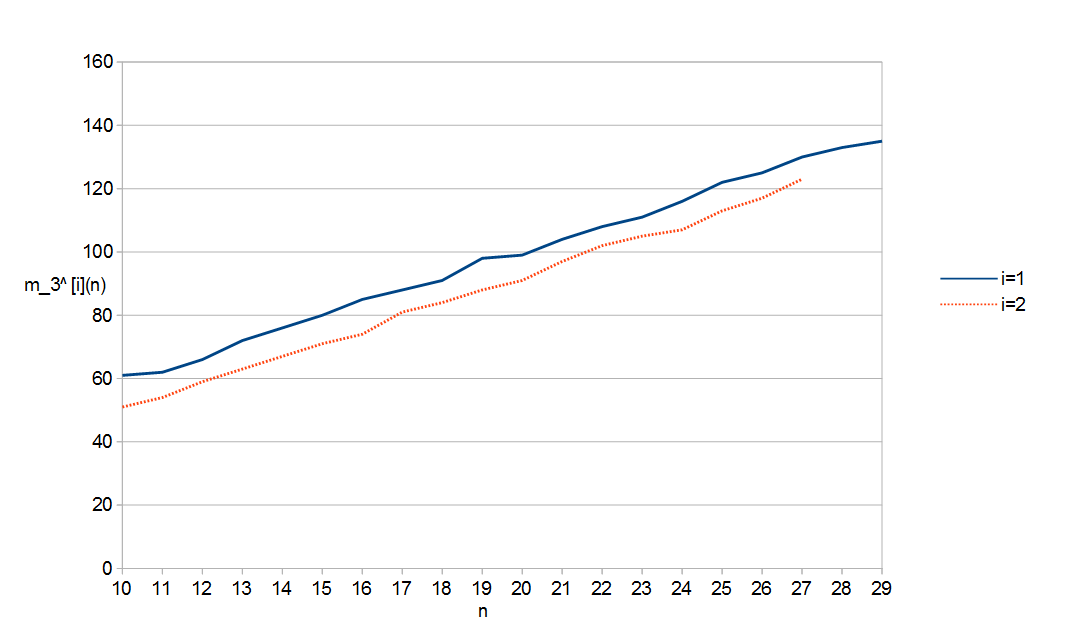
\includegraphics[width=\linewidth]{Diagram.png}
	\caption{Mapping von $n$ zu $m_3^{[i]}(n)$\label{fig:diagram}}
\end{figure}
In unserer Implementierung gilt für Verteilung $[1]$ $n_{max} = 29$ und für Verteilung $[2]$ $n_{max} = 27$.\\
\begin{adjustwidth}{-1cm}{}
\begin{tabular}{l|rrrrrrrrrrrrrrrrrrrr}
	$n$ & 10 & 11 & 12 & 13 & 14 & 15 & 16 & 17 & 18 & 19 & 20 & 21 & 22 & 23 & 24 & 25 & 26 & 27 & 28 & 29\\
	\midrule
	$m_3^{[1]}(n)$ & 61 & 62 & 66 & 72 & 76 & 80 & 85 & 88 & 91 & 98 & 99 & 104 & 108 & 111 & 116 & 122 & 125 & 130 & 133 & 135\\
	\midrule
	$m_3^{[2]}(n)$ & 51 & 54 & 59 & 63 & 67 & 71 & 74 & 81 & 84 & 88 & 91 & 97 & 102 & 105 & 107 & 113 & 117 & 123 & & \\
\end{tabular}
\end{adjustwidth}
\vspace{10pt}
Wie man sieht, gilt durchgängig $m_3^{[1]}(n) > m_3^{[2]}(n)$. Dies haben wir erwartet, da Verteilung $[1]$ auch Klauseln erstellen kann, in denen $x \vee \non{x}$ vorkommt für eine Variable $x$. Dadurch sind Formeln nach Verteilung $[1]$ tendenziell eher erfüllbar. Diese Ergebnisse sind ebenfalls zu sehen in Abbildung \ref{fig:diagram}.

Es ist hierbei ein nahezu linearer Anstieg von $m_3^{[i]}(n)$ erkennbar. Mittels linearer Regression kann die Line of Best Fit bestimmt werden. Diese beträgt:\\
$m_3^{[1]}(n) \approx 18.72+4.07\cdot n$\\
$m_3^{[2]}(n) \approx 8.37+4.19\cdot n$\\
Auf den ersten Blick scheint die Vermutung aus der Aufgabenstellung somit erfüllt zu sein, aber diese impliziert, dass die Line of Best Fit nahe an $(0,0)$ verlaufen müsste, was nicht der Fall ist. Ferner würde hierdurch ab einem $N$ die Ungleichung $m_3^{[1]}(N) < m_3^{[2]}(N)$ gelten, was keinen Sinn ergibt.\par
Falls $m_3^{[1]}(0) = m_3^{[2]}(0) = 0$ verlangt wird, so führt dies zu folgenden Ergebnissen:\\
$m_3^{[1]}(n) \approx 4.94\cdot n$\\
$m_3^{[2]}(n) \approx 4.61\cdot n$\\
Diese führt aber für Verteilung $[1]$ selbst bei großen $n$ zu sehr starken Abweichungen. Für Verteilung $[2]$ hingegen liegen die Ergebnisse \emph{insbesondere} für große $n$ recht nahe an dieser Linie.\par
Somit ist $\tau_3 = 4.61$ ein plausibler Wert für Verteilung $[2]$. Für Verteilung $[1]$ ist der beste Wert $\tau_3 = 4.94$, dieser ist aber auf diesen Ergebnissen nicht besonders gut.

\subsection{3.3b)}
Die Ergebnisse von Aufgabenteil b) sind in Abbildung \ref{fig:b1} und \ref{fig:b2} zu sehen. Auf der Ordinate ist jeweils  $\sigma_3^{[i]}(n_{max},m)$ in Prozent aufgetragen.
\begin{figure}[t]
	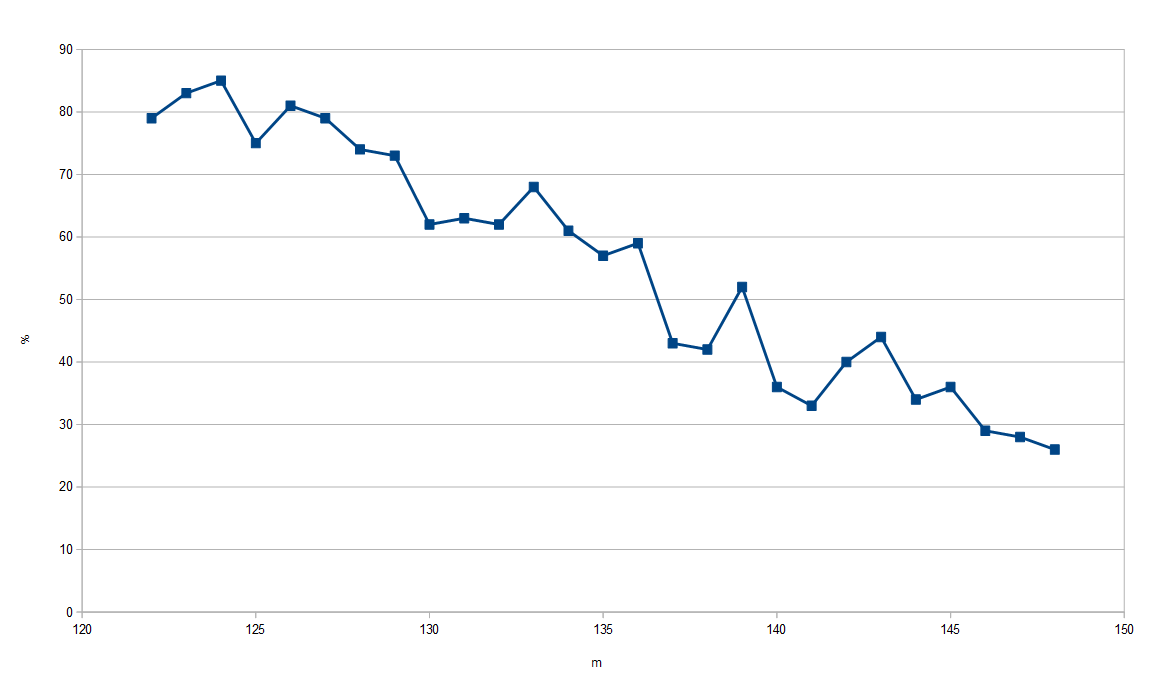
\includegraphics[width=\linewidth]{Diagram-A.png}
	\caption{Verteilung [1] $n_{max} = 29$; $m \in [122,148]$\label{fig:b1}}
\end{figure}
\begin{figure}[t]
	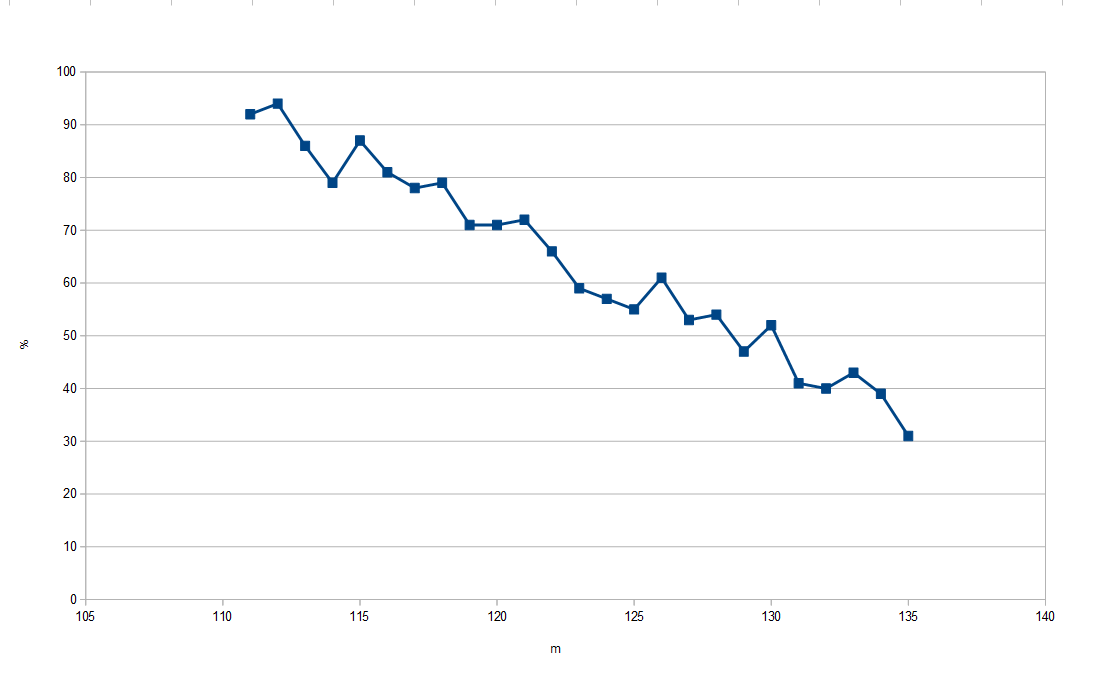
\includegraphics[width=\linewidth]{Diagram-B.png}
	\caption{Verteilung [2] $n_{max} = 27$; $m \in [111,135]$\label{fig:b2}}
\end{figure}
\end{document}